\chapter{Introducción}\label{sec:intro}

\section{Introducción}
\subsection{Motivación y objetivos}
\newpage
\subsection{Planificación (Diagrama de Gantt)}
\begin{center}
	\begin{figure}[H]
		\center
		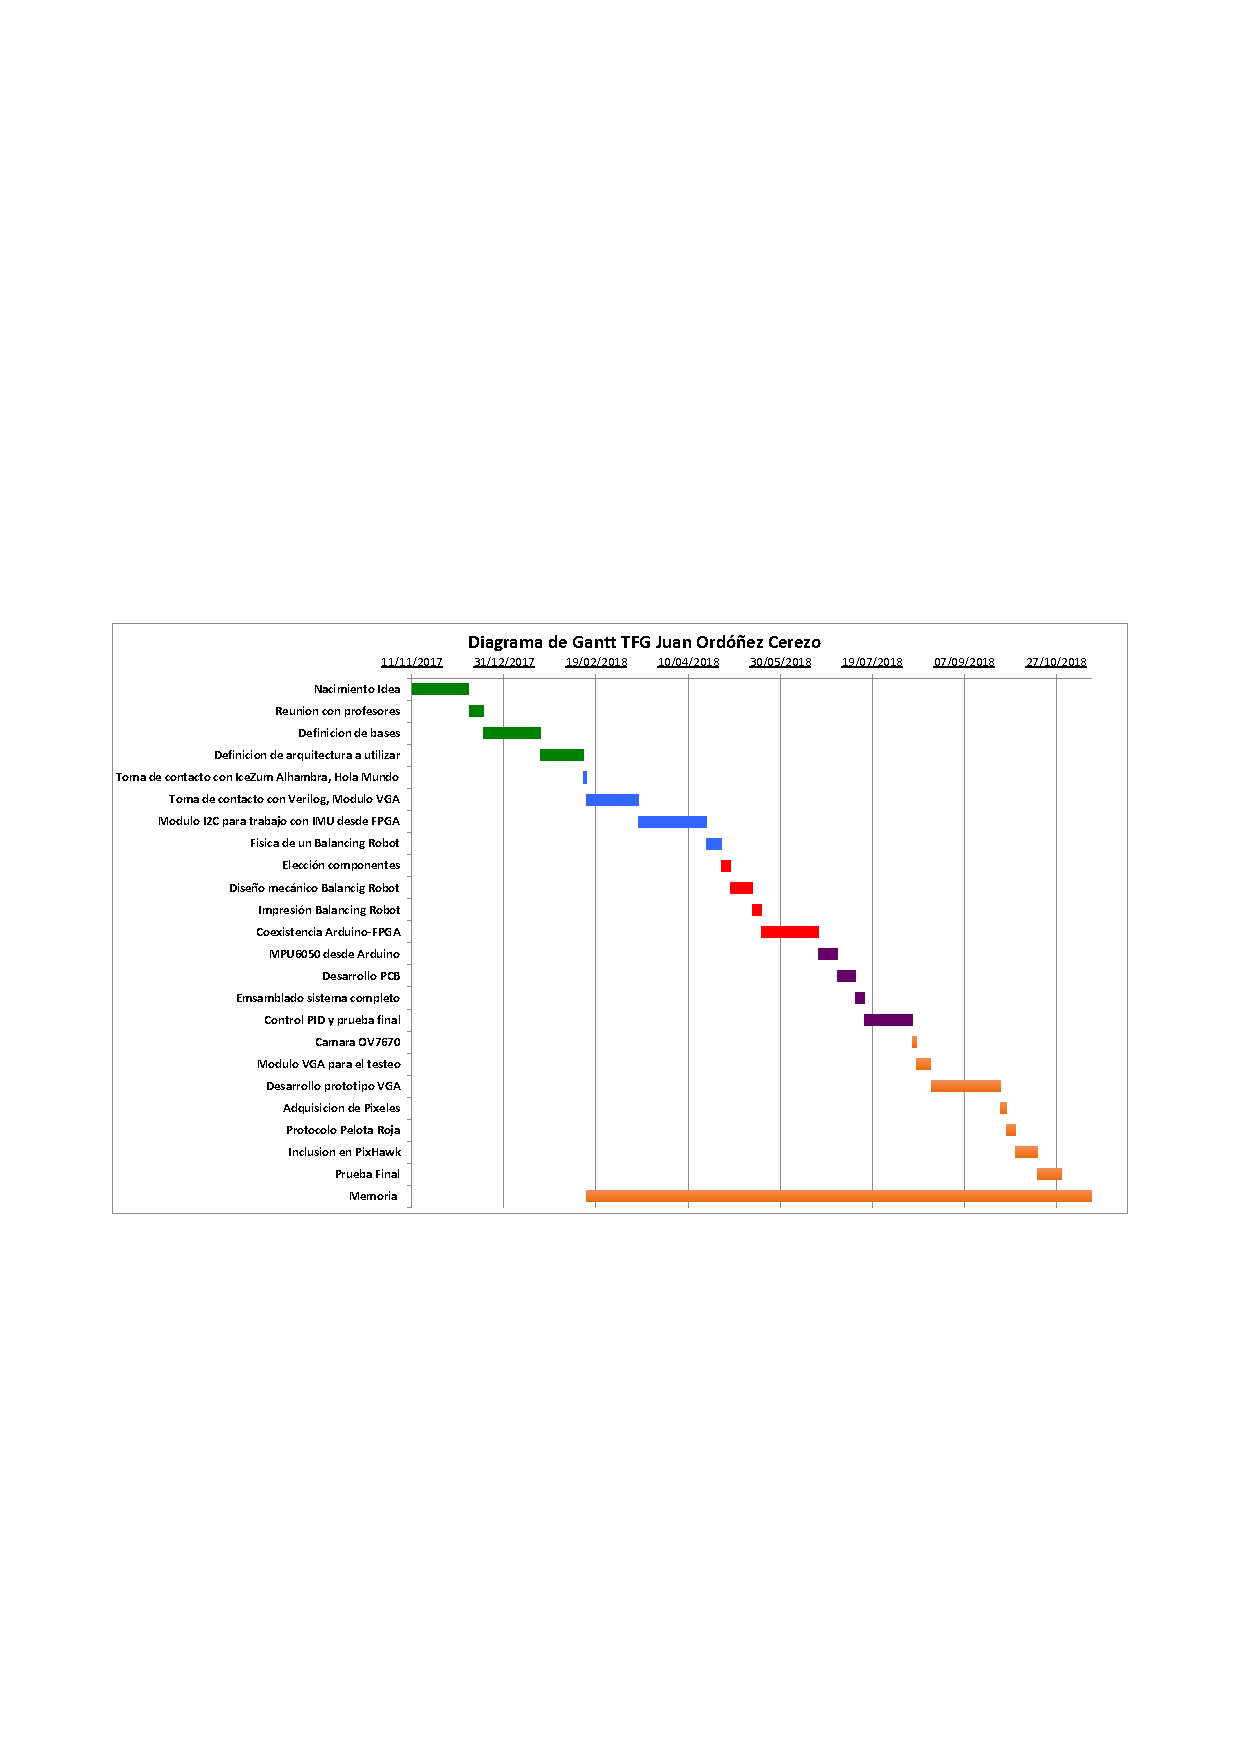
\includegraphics[trim = 15mm 85mm 0mm 100mm,clip, angle=-90, scale = 1.4]{imagenes/Introduction/Gantt.pdf}
		\label{fig:diagramaGantt}
	\end{figure}
\end{center}
\subsection{Metodología de trabajo}
Para explicar la metodología de trabajo seguida, se presenta la herramienta GitHub (figura \ref{fig:github}).\newline 

\begin{figure}[H]
	\center
	
\includegraphics[trim = 0mm 0mm 0mm 0mm, clip,scale=0.4]{imagenes/Introduction/github}
	\caption{Logo GitHub.}
	\label{fig:github}
\end{figure}


GitHub es una plataforma de desarrollo colaborativo de software para alojar proyectos utilizando el sistema de control de versiones Git. GitHub aloja tu proyecto en un repositorio y brinda herramientas muy útiles para el trabajo en equipo. \newline
Proporciona además la posibilidad de una Wiki para el mantenimiento de las versiones e información acerca de ellas. \newline
En el presente proyecto GitHub ha sido usado como un contenedor, donde se ha ido subiendo todo de manera parcial, normalmente, cuando se obtenía una versión estable sobre algunas de las ramas. \newline
De esta forma, y al ser abierto, cualquier persona ha podido seguir los avances de este, dudas, problemas, o incluso utilizar algunos de los módulos o material subidos. \newline
 
El proyecto puede encontrarse en la siguiente URL: \newline

\hyperref[]{https://github.com/RoboticsURJC-students/2017-tfg-juan-ordonez}

Un ejemplo de la trayectoria de este proyecto se representa en la captura de pantalla de GitHub en la figura \ref{fig:capturaGit}.

\begin{figure}[H]
	\center
	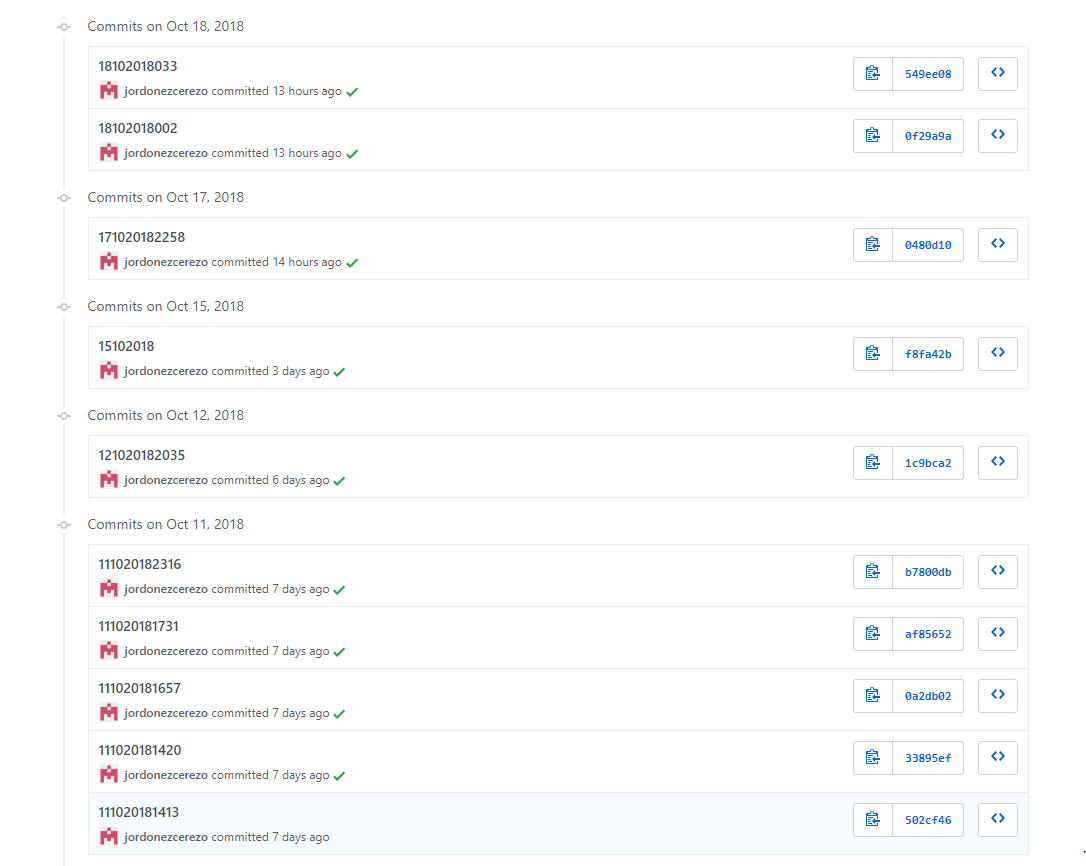
\includegraphics[trim = 0mm 0mm 0mm 0mm, clip,scale=0.5]{imagenes/Introduction/CapturaGit}
	\caption{Commits GitHub.}
	\label{fig:capturaGit}
\end{figure}

Para el buen cumplimiento de los objetivos planteados en primera instancia, y teniendo en cuenta la diferente localización de los componentes del trabajo, se hizo necesario el planteamiento de reuniones semanales (normalmente los Viernes) donde se pusiese en común lo trabajado durante la semana y se fijasen los siguientes objetivos. \newline

Para ello, se utilizo la herramienta se software libre llamada "Appear.in", la cuál ofrece videoconferencias entre varios usuarios al mismo instante (figura \ref{fig:appear}). 

\begin{figure}[H]
	\center
	
\includegraphics[trim = 0mm 0mm 0mm 0mm, clip,scale=0.3]{imagenes/Introduction/appear}
	\caption{Appear.in.}
	\label{fig:appear}
\end{figure}

\subsection{Estructura de la memoria}